% ---------------------------------------------
%              _ 
%  _ __   ___ | |_   _  __ _  ___  _ __  ___
% | '_ \ / _ \| | | | |/ _` |/ _ \| '_ \/ __| /\/|
% | |_) | (_) | | |_| | (_| | (_) | | | \__ \|/\/
% | .__/ \___/|_|\__, |\__, |\___/|_| |_|___/
% |_|            |___/ |___/
% ---------------------------------------------
%*!     wc: 943
%**     wc: 2000
%*[ ]   Make Github Page
%*[ ]   Tidy Pd patches - rename click+-
%*[ ]   Tidy .cs scripts
%*[ ]   Link fig: to github scripts
%*[x]   Decide on chapter sections
%*[x]   Draft summary
%*[X]   Draft composition
%*[ ]   Draft performance write up
%*[ ]   Draft demo write up
%*[ ]   Draft future
% ---------------------------------------------
\chapter{Performing polygons\textasciitilde{}}
\label{sec: polygons}
\markboth{}{Performing polygons\textasciitilde{}}
\epigraph{\emph{quote}}{\citep[]{bilbow2022}}
% ---------------------------------------------
\begin{figure}
    \centering
    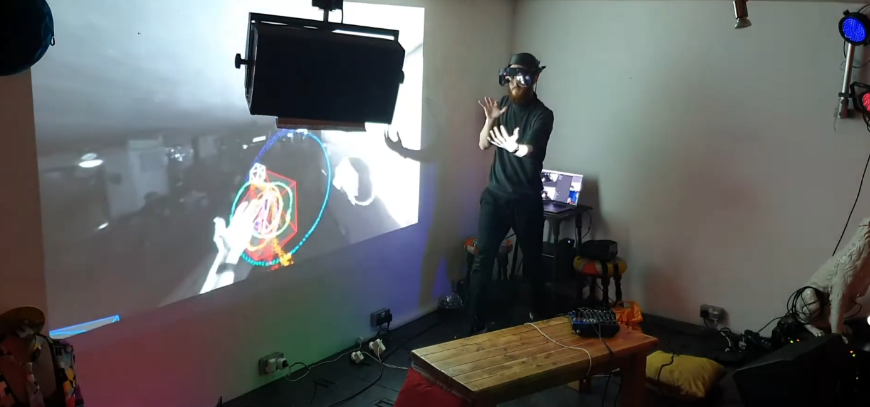
\includegraphics[width=0.7\linewidth]{07-polygons/polygons-ambi-rh.png}
    \caption{Performance of \textit{polygons\textasciitilde{}} at The Rosehill}
    \label{fig: polygons-ambi-rh}
\end{figure}
\section{Developing an AR Performance Practice} \label{sec: polygons-developing}
As a direct consequence of witnessing participants enjoyment and play with \textit{polaris\textasciitilde{}}, I recognised for the first time looking from the outside in, that the system had a larger propensity for fostering learning, virtuosity, and depth of expression than I had originally thought; if only the experience was slightly more complex, the interactions more \textit{nuanced}. The gestures, play, and expression by participants led to a kind of quasi-transhumanist dance, one that struck me as a technologically mediated dialogue between hybrid self and hybrid environment, a delicate balance of agency.

Until this point, I had been primarily focused on the medium as used for the composition of musical pieces e.g. \hyperref[sec: area]{\textit{area\textasciitilde{}}}, or of installation-like experiences \hyperref[sec: polaris]{\textit{polaris\textasciitilde{}}}. Performance with AR had remained abstract, especially as, formally, its not my preferred mode of musical expression. However, the balance of agency between participant and system, between self and environment, presented itself during the evaluation of \textit{polaris\textasciitilde{}} to be an area ready for exploration through performance. 

Most of the software and hardware I had used in the development of \textit{polaris\textasciitilde{}} was readily transferable to the context of performance. There was no need to change from the combination of PureData, LibPdIntegration, and Unity. However, performance did confront me with new considerations: 
\begin{itemize}
    \item \textit{What elements of my experience would need to be shared with an audience?} 
    \item \textit{What role would my gestures have in describing the experience that I was by now intimately aware of, but would be strange for an audience?} 
\end{itemize}
The following chapter outlines my exploration of a a fifteen-minute experimental audiovisual AR improvisation using an AR performance ecosystem called \textit{Weird Polygons and Hand Noises}, or \textit{polygons\textasciitilde{}} for short.



% ---------------------------------------------
\section{The Composition of Weird Polygons and Hand Noises} \label{sec: polygons-composition}

Drawing from the categories extracted from \nameref{sec: polaris}: \nameref{sec: polaris-feedback}, I pursued the design of a system with physically moveable elements, audio-reactivity, and enough room to be able to learn and explore the scene both spatially and in terms of interaction and sonic palette. Thus, as an AR performance ecosystem, \textit{polygons\textasciitilde{}} delivers this by describing the improvisational and performative relationship between a performers actions via body, hand, and head movement, feedback from the audience, and three real-time AR musical instruments: \textit{ambi}, \textit{click}, and \textit{hands}. 

%*[ ]   add unity image of ambi w/ particles
\textit{ambi}, a red wireframe icosahedron, serves as a dual-oscillator drone synthesiser that the performer can call on my taking and bringing it closer to them with their hands. Its voice is contingent eleven real-time parameters, which are sent to the PureData patch attached to it. At specified distance two particle systems are activated from the palms of the performers hands, and the drone from \textit{ambi} is activated. The particles are drawn to the centre of \textit{ambi}, their paths guided by an unseen particle forcefield - the same behaviour as in \textit{polaris\textasciitilde{}}. Real-time hand `collision' in three dimensions with \textit{ambi} is constantly reported per hand, resulting in two sets of $x,y,z$ coordinates that form part of the data that is mapped to parameters in PureData (see \autoref{fig: polygons-ambi-mapping}).
\begin{table}
    \centering
    \begin{tabular}{ l|l l }
        \textbf{Unity Scene Attribute}  & \multicolumn{2}{ l }{\textbf{PureData Parameter}}   \\
        \hline
        \textbf{Hand}                   & \textbf{via Left Hand}& \textbf{via Right Hand}       \\
        \hline
        Collision Distance              & Drone 1 On / Off      & Drone 2 On / Off              \\
        Collision X                     & Reverb Amount         & Drone 2 LPF CF Mod            \\
        Collision Y                     & Drone 1 Pitch         & Drone 2 Pitch                 \\
        Collision Z                     & Rev/Dly Amount        & Drone 2 LPF CF                \\
        \hline
        
        \textbf{\textit{ambi}}          & \multicolumn{2}{ l }{\textbf{via pinch gesture}}    \\
        \hline
        Scale                           & \multicolumn{2}{ l }{Output Filter Cutoff}          \\  
    \end{tabular}
    \caption{The parameter mappings for \textit{ambi}}
    \label{fig: polygons-ambi-mapping}
\end{table}
%*[ ]   move panel in patch under each other for space
\begin{figure}
    \centering
    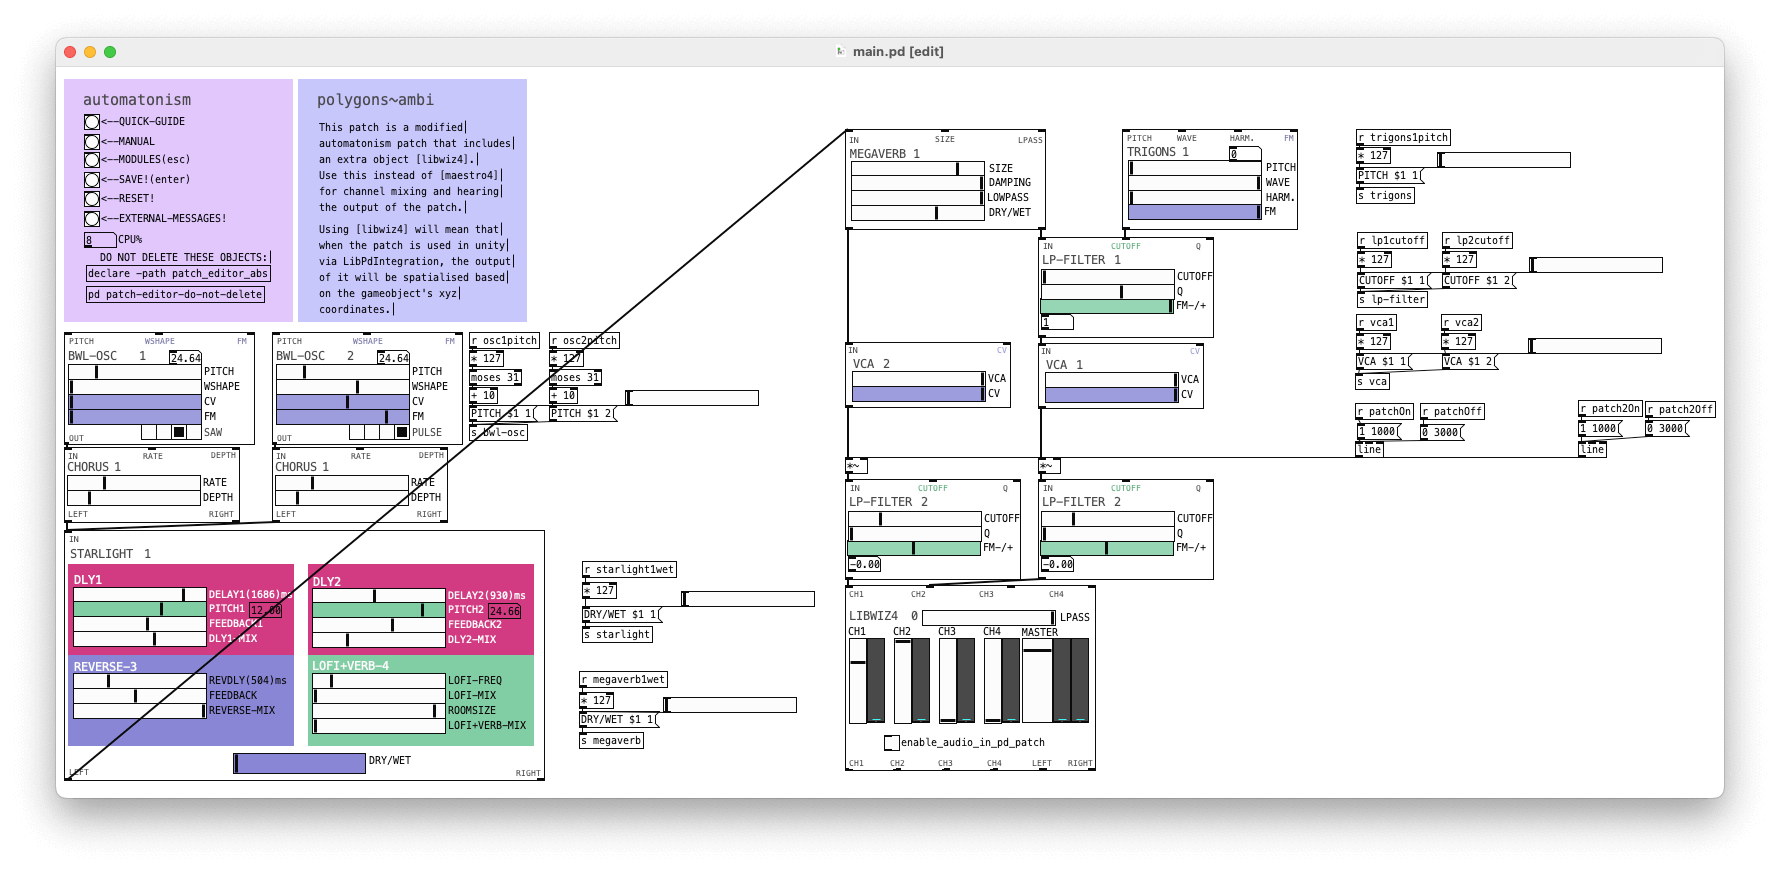
\includegraphics[width=0.7\linewidth]{07-polygons/polygons-ambi-pd.png}
    \caption{The PureData patch for \textit{ambi}}
    \label{fig: polygons-ambi-pd}
\end{figure}

%*[ ]   add unity image of click w/ particles
\textit{click}, a set of two blue wireframe icosahedra, form a feedback system between two low-frequency oscillator controlled impulse generators. The feedback can be altered by bringing the smaller icosahedron (\textit{click-}) closer to the larger one (\textit{click+}). \textit{click+-} makes use of LibPdIntegration's Unity send functionality; each time there is an impulse generated, a message is sent to Unity, which triggers a shower of particles to be emitted from \textit{click-} to \textit{click+} forcefield-guided cone. As the performer intervenes and creates the feedback system, the closer they bring the icosahedra together, the faster the visual particle shower becomes, and the more erratic the impulse generators feedback on each other. A further sound parameter, connected to a reverb, is mapped to the amount spin \textit{click-} let go with by the performer. The sound palette explores a gradient from static electricity crackles to a sound akin toa car motor catching and revving up as the feedback increases.
\begin{table}
    \centering
    \begin{tabular}{ l|l }
        \textbf{Unity Scene Attribute}         & \textbf{PureData Parameter}   \\
        \hline      
        \textit{click+-} Distance              & Impulse 1 Frequency           \\
        \textit{click-} Collision X            & Impulse 2 Frequency           \\
        \textit{click-} Collision Y            & Impulse Chorus Rate           \\
        \textit{click-} Collision Z            & Impulse Chorus Depth          \\
        \textit{click-} Release Spin Velocity  & Impulse Reverb Amount     
    \end{tabular}
    \caption{The parameter mappings for \textit{click}}
    \label{fig: polygons-click-mapping}
\end{table}
\begin{figure}
    \centering
    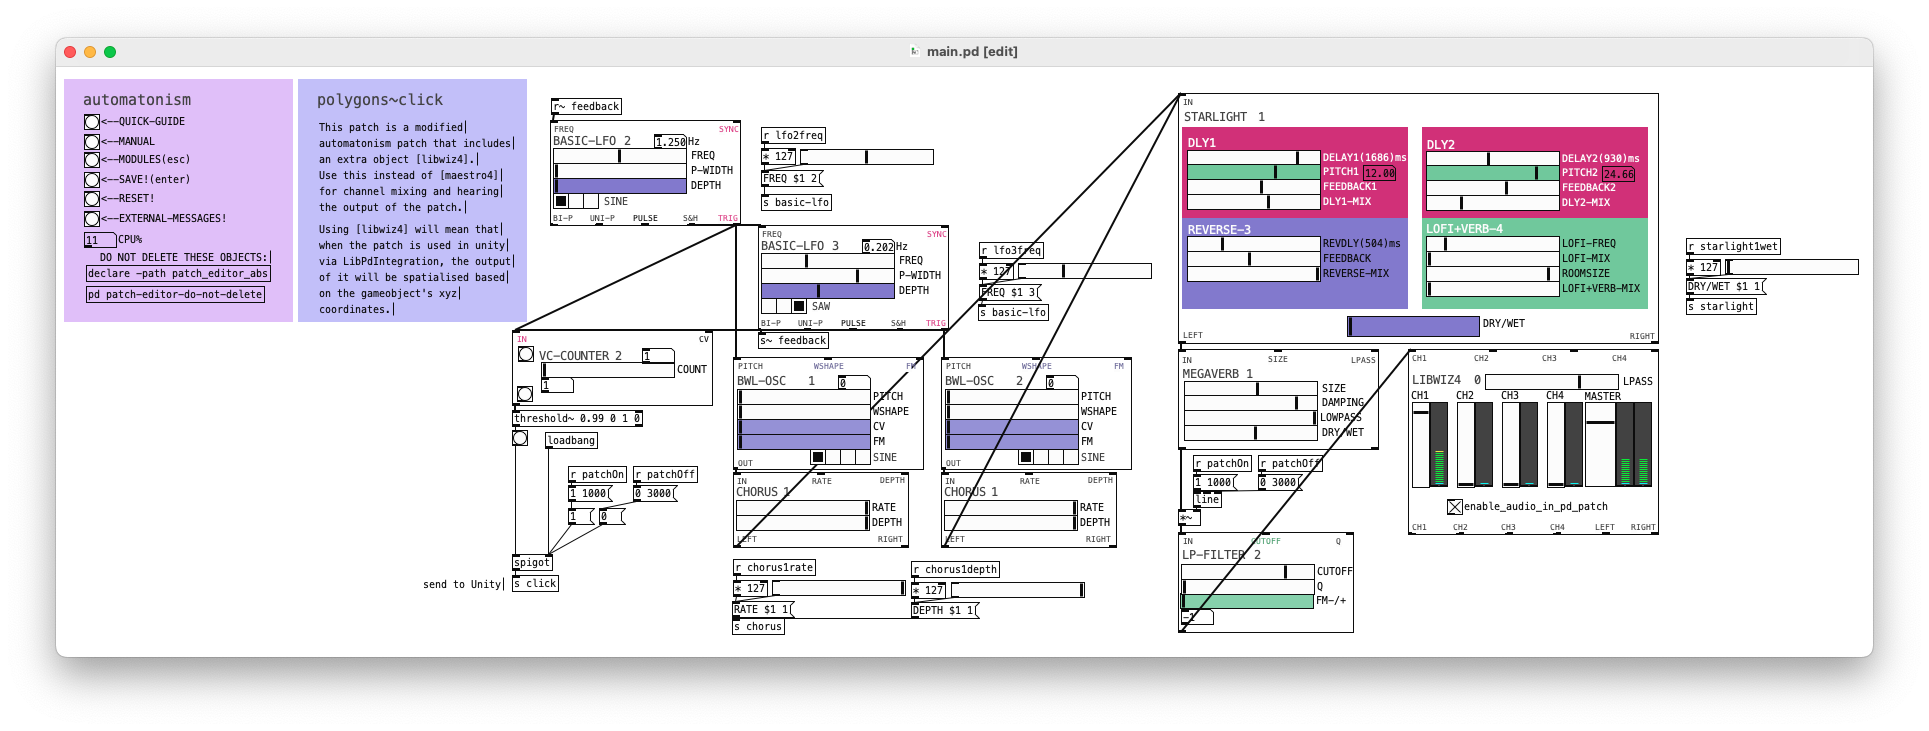
\includegraphics[width=0.7\linewidth]{07-polygons/polygons-click-pd.png}
    \caption{The PureData patch for \textit{click}}
    \label{fig: polygons-click-pd}
\end{figure}

%*[ ]   add unity image of hand w/ colours
\textit{hands} constitutes the final AR instrument in \textit{polygons~}; each of the performers hands, when a virtual button besides their palm is toggled \textit{on}, generate a highly resonant filtered white noise. The cutoff, resonance, and amplitude of this generator-filter system is controllable independently per hand, through several dynamic movement-based attributes. The filter cutoff per hand is linearly mapped to that hand's distance to the performers face; the filter resonance per hand is mapped to the angle from that hand's palm angle towards the centre of the performance space; and the amplitude of each is mapped to the stretching of the fingers outwards away from the palm. The sounds delivered by \textit{hands} are harsh and unpleasant at certain parameter combinations and purposefully loud; from a performative standpoint, this engenders specific gestures, movements, and stances, as the performer grapples with a sonic experience akin to howling and shrieking winds.
\begin{table}
    \centering
    \begin{tabular}{ l|l }
        \textbf{Unity Scene Attribute}         & \textbf{PureData Parameter}    \\
        \hline      
        \textit{hand} to Head Distance         & Filter Cutoff                  \\
        \textit{hand} to Stage Angle           & Filter Resonance               \\
        \textit{hand}'s Finger Extension       & Amplitude               
    \end{tabular}
    \caption{The parameter mappings for \textit{hands}}
    \label{fig: polygons-hands-mapping}
\end{table}
\begin{figure}
    \centering
    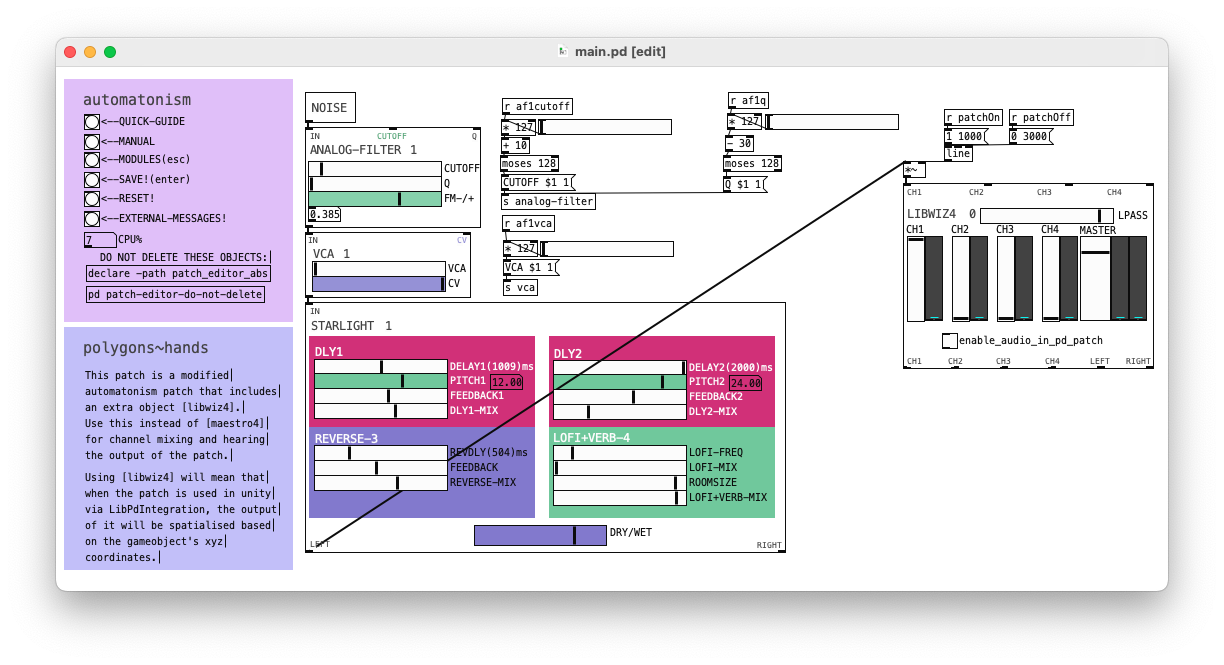
\includegraphics[width=0.7\linewidth]{07-polygons/polygons-hands-pd.png}
    \caption{The PureData patch for \textit{hands}}
    \label{fig: polygons-hands-pd}
\end{figure}

Together, and separately, \textit{ambi}, \textit{click-+}, and \textit{hands} provide a complex sound palette, explorable by the performer through non-linear combinations of hand gestures, body movements, and stances, that themselves invariably feed back into the decisions made to delve into specific sounds. Visually, \textit{polygons\textasciitilde{}} draws on the primitive wireframe AR systems of the early 20th century such as the \textit{KARMA} system \cite{feiner1993} and Sutherland's \textit{Ultimate DIsplay} \citep{sutherland1968} (see: \autoref{fig: polygons-wireframes}), which were constrained by computer power. This is juxtaposed by the fluid and visually complex behaviour of the thousands of multicoloured particles used by \textit{ambi}, and \textit{click-+}.

\begin{figure}
    \centering
    \subcaptionbox{Sutherlands `Ultimate Display'}[.3\linewidth]{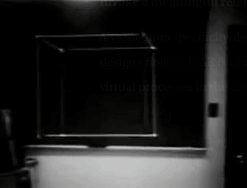
\includegraphics[height=2.5cm]{07-polygons/sutherland_68.png}}
    \hfill
    \subcaptionbox{Feiner's `KARMA' System}[.3\linewidth]{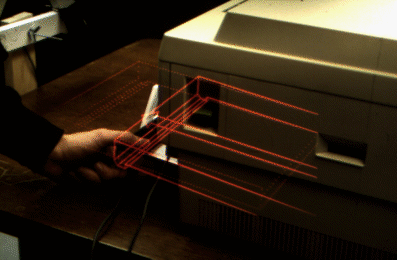
\includegraphics[height=2.5cm]{07-polygons/feiner_93_2.png}}%
    \caption{Wireframe Influences}
    \label{fig: polygons-wireframes}
\end{figure}


% ---------------------------------------------
\section{Performances} \label{sec: polygons-performances}
\subsection{Technical Setup} \label{sec: polygons-performances-setup}
%*? Laptop?
%*? Method of audience display -> 2x headset -> laptop -> projector
%*? Speaker reversal

\subsection{emute\_06 at The Rosehill} \label{sec: polygons-performances-rosehill}
polygons\textasciitilde{} was developed for a performance as part of the seventh Experimental Music Technologies (emute) Lab \href{http://www.emutelab.org/blog/emutelab6}{showcase} at The Rosehill - an independent venue, recording studio, label, creative hub and co-working space run by artists and musicians.

\subsection{Showcase at the ACCA} \label{sec: polygons-performances-acca}



% ---------------------------------------------
\section{Demonstrations} \label{sec: polygons-demonstrations}
\subsection{MAH Doctoral Conference} \label{sec: polygons-demonstrations-mah}

\subsection{SHL Make \& Create} \label{sec: polygons-demonstrations-shl}

\subsection{Embodiment Hackathon} \label{sec: polygons-demonstrations-emh}



% ---------------------------------------------
\section{The Future of AR Musical Performance}
\subsection{Intimacy}
\subsection{Relevant Work}
%** Green, Hayes, guy from TAP, guy from PNS, guy from YT
\subsection{Moving forwards}